\documentclass[runningheads]{llncs}

\usepackage[T1]{fontenc}
\usepackage{graphicx}
\usepackage{booktabs}
\usepackage{multirow}
\usepackage{amsmath}
\usepackage{url}
\setlength{\textfloatsep}{8pt plus 1pt minus 2pt}
\setlength{\floatsep}{8pt plus 1pt minus 2pt}
\setlength{\intextsep}{8pt plus 1pt minus 2pt}

\begin{document}

\title{RaOD-ERAS: Road-Prototype Anomaly Heatmap with Ego-Lane Risk-Aware Refinement for Unexpected Road Obstacle Segmentation}
\titlerunning{RaOD-ERAS for Road Anomaly Segmentation}

% METADATA_START
\author{First Author\inst{1} \and Second Author\inst{1} \and Corresponding Author\inst{1}}
\authorrunning{F. Author et al.}
\institute{Institution Name, City, Country\\
\email{author@example.com}}
% METADATA_END

\maketitle

\begin{abstract}
Unexpected road obstacles such as animals, debris, and other rare objects pose safety risks for intelligent vehicles because they are often under-represented in closed-set perception training data. This paper presents RaOD-ERAS, a lightweight training-free framework for unexpected road obstacle segmentation. The method uses pretrained DINOv2 visual features to construct a road-prototype anomaly heatmap and then applies Ego-lane Risk-Aware Segmentation (ERAS), which combines road-region, ego-lane, near-field, and connected-component risk priors. The final output includes an interpretable anomaly heatmap, a binary anomaly mask, and structured warning events that can be consumed by a downstream safety module. Experiments on SMIYC RoadObstacle, RoadAnomaly21, and a 149-sample StreetHazards partial subset show that the proposed refinement improves AP and FPR95 on SMIYC, improves F1/IoU/FPR95 under RoadAnomaly21 domain shift, and reduces false positives on the difficult StreetHazards partial subset. The results indicate that road-prototype features and risk-aware refinement are useful for fast conference-level road anomaly studies, while also revealing limitations under strong synthetic-domain shift.

\keywords{Road anomaly segmentation \and Intelligent vehicles \and DINOv2}
\end{abstract}

\section{Introduction}

Autonomous and assisted driving systems must react to rare and unexpected road objects. In contrast to common traffic participants, anomalous obstacles may not belong to the label set used by a perception model. This creates a need for anomaly segmentation methods that can highlight unknown objects and provide actionable warning outputs.

Existing benchmarks such as SegmentMeIfYouCan evaluate anomaly segmentation in road scenes~\cite{chan2021segmentmeifyoucan}, and prior methods such as DiCNet~\cite{tian2022dicnet} and PEBAL~\cite{tian2022pebal} study stronger supervised or benchmark-oriented solutions. In this work, we focus on a practical small-conference setting: no new supervised model is trained, but a reproducible road anomaly pipeline is built from pretrained visual features and explicit road-scene priors.

The contributions are as follows. First, we build a DINOv2-based road-prototype anomaly heatmap by comparing image patches against normal road-region features. Second, we propose ERAS, an ego-lane risk-aware refinement module that calibrates heatmaps using road, lane, near-field, and connected-component cues. Third, we export structured warning events from the final binary mask, connecting perception output to downstream safety monitoring. Fourth, we report experiments on three public road anomaly datasets or subsets with an explicit claim boundary.

\section{Related Work}

\subsection{Road Anomaly Segmentation}
SegmentMeIfYouCan provides a benchmark for anomaly segmentation in road scenes~\cite{chan2021segmentmeifyoucan}. It motivates methods that detect unknown obstacles beyond the closed-set semantic classes used by conventional segmentation. RoadAnomaly21 and SMIYC RoadObstacle are therefore suitable for evaluating unexpected road object segmentation.

\subsection{OOD Detection in Driving Scenes}
StreetHazards is a synthetic benchmark for out-of-distribution object detection in urban driving scenes~\cite{hendrycks2019scaling}. It is harder to compare directly with SMIYC because of domain shift and label format differences. In this paper, the available partial StreetHazards subset is used only as a difficult-domain supplement, not as a complete official benchmark result.

\subsection{Foundation Features}
DINOv2 learns strong self-supervised visual representations~\cite{oquab2023dinov2}. We use it as a frozen feature extractor. Unlike supervised anomaly segmentation methods, the proposed pipeline does not optimize model weights on the target anomaly datasets.

\section{Method}

\subsection{Road-Prototype Anomaly Heatmap}
Given an RGB road image, DINOv2 extracts patch-level feature embeddings. A simple trapezoid-shaped road prior selects likely normal road patches. Their average feature vector is used as a road prototype. The anomaly score of each patch is computed from its distance to the road prototype and then upsampled to the original image resolution.

\subsection{ERAS Refinement}
The initial heatmap may highlight background textures or distant regions. ERAS refines it using four priors: road-region prior, ego-lane prior, near-field weighting, and connected-component risk scoring. The refined heatmap is normalized and converted into a binary mask using the threshold selected during evaluation.

\begin{figure}
  \centering
  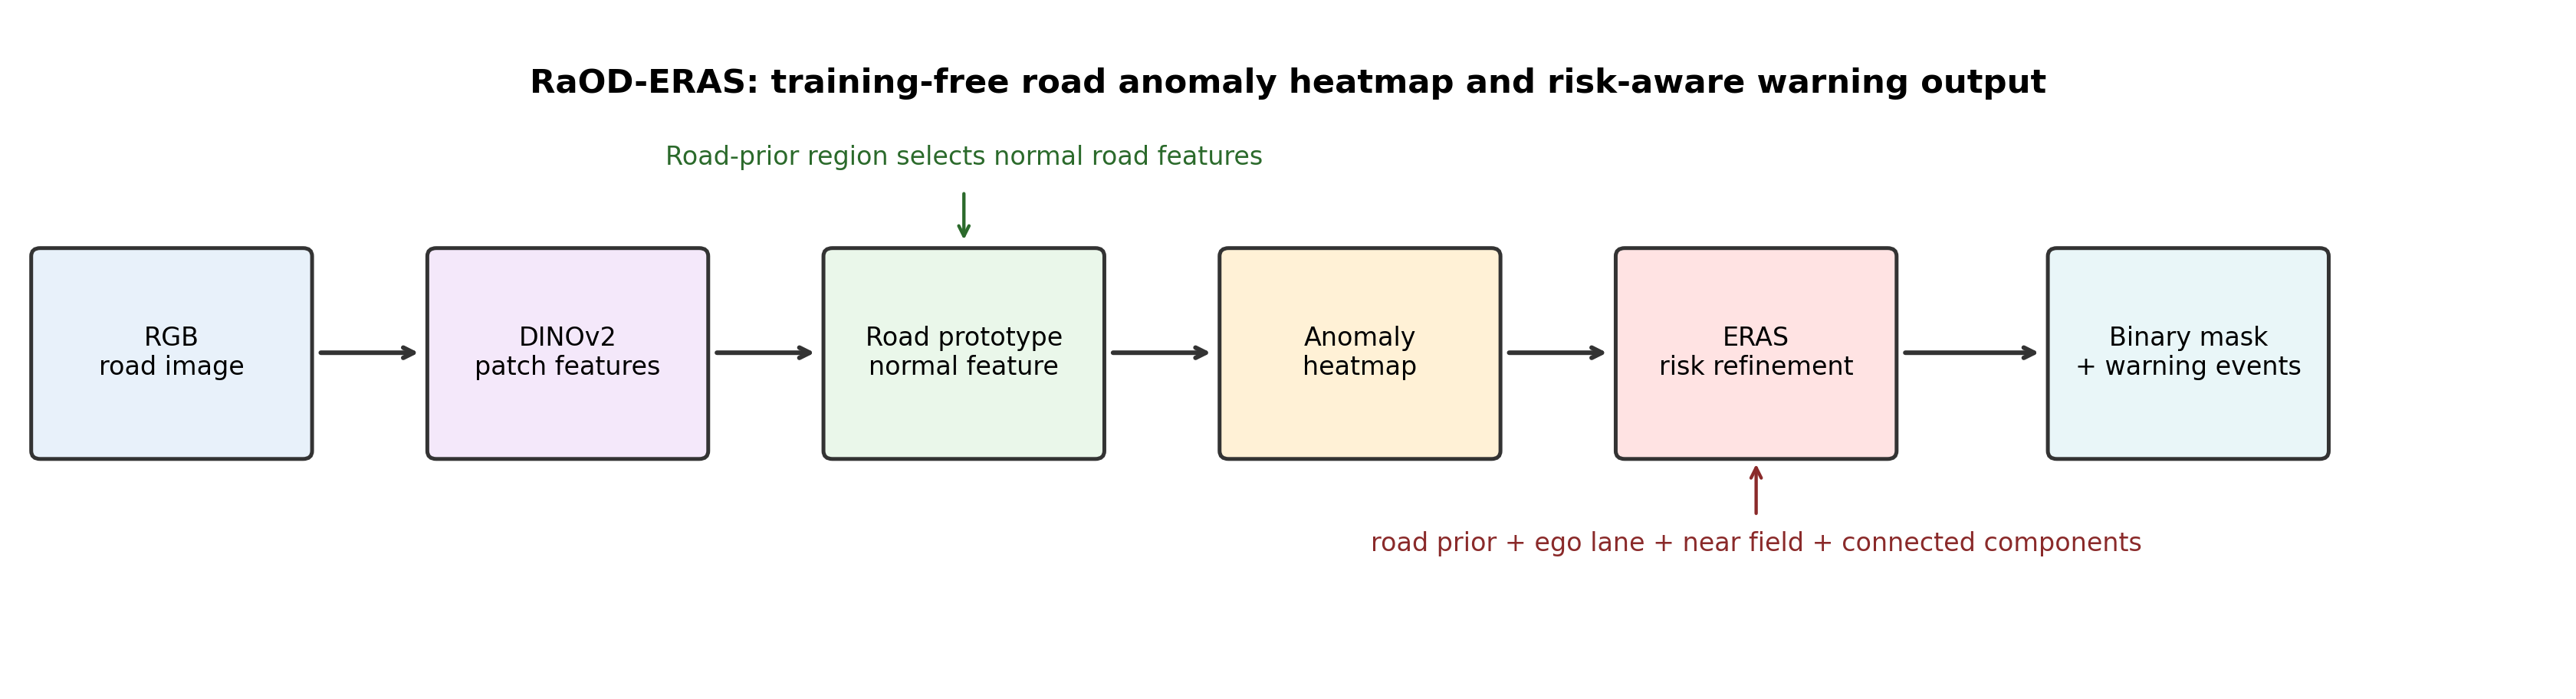
\includegraphics[width=0.86\linewidth]{figures/framework_pipeline.png}
  \caption{Overview of RaOD-ERAS. DINOv2 features produce a road-prototype anomaly heatmap; ERAS converts it into a risk-aware binary mask and structured warning events.}
  \label{fig:pipeline}
\end{figure}

\subsection{Warning Event Output}
The final thresholded mask is decomposed into connected components. Each component is assigned a bounding box, area, mean heatmap score, road overlap, lane overlap, near-field weight, and risk score. The resulting JSONL event can be passed to a downstream warning or slow-down module.

\section{Experiments}

\subsection{Datasets and Metrics}
We evaluate on SMIYC RoadObstacle, RoadAnomaly21, and a 149-sample StreetHazards partial subset extracted from an interrupted test archive. Metrics include AP, F1, IoU, precision, recall, and FPR95. AP evaluates heatmap ranking quality, F1 and IoU evaluate binary mask quality, and FPR95 reflects false-positive behavior at high recall.

\subsection{Quantitative Results}

Tables~\ref{tab:smiyc}--\ref{tab:streethazards} summarize the quantitative evidence for the training-free setting.

\begin{table}
\centering
\small
\caption{SMIYC RoadObstacle results on 30 public GT images.}
\label{tab:smiyc}
\begin{tabular}{lrrrrrr}
\toprule
Method & AP & F1 & IoU & Prec. & Rec. & FPR95 \\
\midrule
RoadContrast & 0.1169 & 0.1739 & 0.1108 & 0.1428 & 0.3690 & 0.4540 \\
RoadContrast + ERAS recall & 0.2180 & 0.2751 & 0.2068 & 0.3456 & 0.3981 & 0.4536 \\
DINO road prototype & 0.5203 & 0.5228 & \textbf{0.3998} & \textbf{0.4781} & 0.6864 & 0.0268 \\
DINO + ERAS light & \textbf{0.5271} & \textbf{0.5232} & 0.3989 & 0.4693 & 0.7524 & \textbf{0.0256} \\
\bottomrule
\end{tabular}
\end{table}

\begin{table}
\centering
\small
\caption{RoadAnomaly21 results on 10 public GT images.}
\label{tab:roadanomaly}
\begin{tabular}{lrrrrrr}
\toprule
Method & AP & F1 & IoU & Prec. & Rec. & FPR95 \\
\midrule
RoadContrast & 0.3698 & 0.4473 & 0.3059 & 0.4022 & 0.6188 & 0.6409 \\
RoadContrast + ERAS balanced & \textbf{0.3733} & 0.4534 & 0.3099 & \textbf{0.4230} & 0.6137 & 0.6191 \\
DINO road prototype & 0.1324 & 0.3119 & 0.1907 & 0.1924 & \textbf{0.9314} & 0.6749 \\
DINO + ERAS balanced & 0.3227 & \textbf{0.4782} & \textbf{0.3289} & 0.3640 & 0.8369 & \textbf{0.5592} \\
\bottomrule
\end{tabular}
\end{table}

\begin{table}
\centering
\small
\caption{StreetHazards partial results on 149 available image/GT pairs. This is not an official complete benchmark result.}
\label{tab:streethazards}
\begin{tabular}{lrrrrrr}
\toprule
Method & AP & F1 & IoU & Prec. & Rec. & FPR95 \\
\midrule
RoadContrast & 0.0295 & 0.0634 & 0.0343 & 0.0421 & 0.4158 & 0.6656 \\
DINO road prototype & \textbf{0.1133} & \textbf{0.1588} & \textbf{0.0975} & \textbf{0.1424} & 0.4781 & 0.3671 \\
DINO + ERAS light & 0.0691 & 0.1344 & 0.0753 & 0.1077 & 0.5177 & \textbf{0.2688} \\
DINO + ERAS balanced & 0.0626 & 0.1293 & 0.0722 & 0.1013 & 0.5432 & 0.2769 \\
\bottomrule
\end{tabular}
\end{table}

\subsection{Qualitative Result}

\begin{figure}
  \centering
  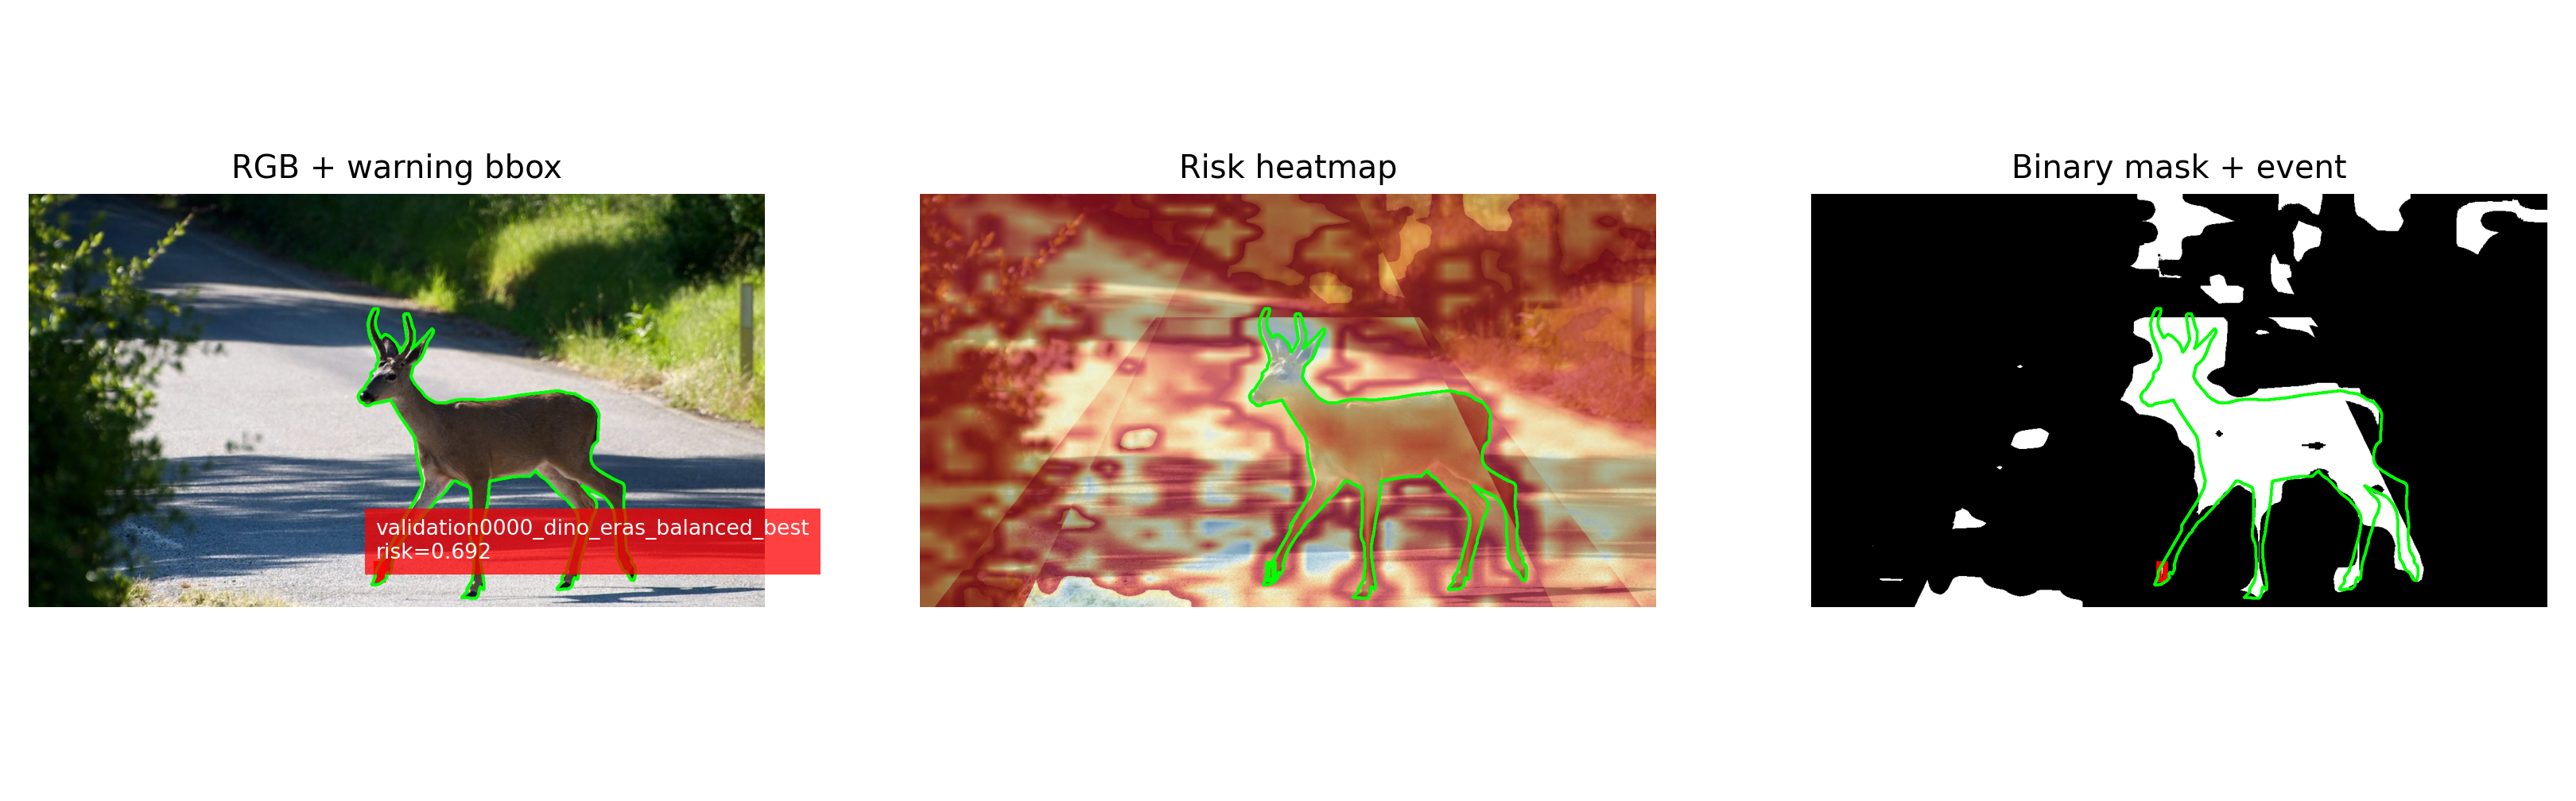
\includegraphics[width=0.86\linewidth]{figures/warning_event_example.png}
  \caption{Example output: RGB warning box, risk heatmap, and binary mask. The green contour denotes GT.}
  \label{fig:warning}
\end{figure}

\section{Discussion}

On SMIYC RoadObstacle, DINO road-prototype heatmaps are already strong and ERAS light slightly improves AP and FPR95. On RoadAnomaly21, raw DINO suffers from domain shift, while ERAS balanced improves F1, IoU, and FPR95. On StreetHazards partial, raw DINO obtains better AP and F1, while ERAS light reduces FPR95. This suggests that ERAS is better understood as a risk-aware calibration and warning-output module, not as a universal accuracy booster.

\section{Limitations}

The public GT subsets of SMIYC and RoadAnomaly21 are small. StreetHazards was only partially downloaded, and the reported 149-sample result is not an official benchmark number. The method relies on geometric road priors and may fail under unusual camera viewpoints or non-road scenes. It also does not replace supervised anomaly segmentation models.

\section{Conclusion}

This paper introduced RaOD-ERAS, a training-free framework for unexpected road obstacle segmentation. It combines DINOv2 road-prototype anomaly heatmaps with ego-lane risk-aware refinement and exports heatmaps, binary masks, and structured warning events. Experiments across three datasets show useful behavior under several settings, while also revealing clear limitations under synthetic-domain shift.

% ACKNOWLEDGEMENTS_START
% ACKNOWLEDGEMENTS_END

\bibliographystyle{splncs04}
\bibliography{references}

\end{document}
